
\subsection{Entities Mobility Models}

An Entity Mobility Model is a Mobility Model that represent mobile nodes whose movements are independents of each other.


\subsubsection{Random Direction}

The Random Waypoint Mobility Model produces a clustering of nodes near the center of the simulation area (see the figure \ref{RandomWaypointFig}). To overcome this problem, the Random Direction Mobility Model was created to ensure an almost constant number of nodes throughout the area simulation. 
In this model, a Mobility Nodes (MNs) chooses a random destination and he will travel to this in order to achieve the border of the simulation area. When a MN reaches a simulation boundary, he pauses for a time specified by the simulation. Then he chooses an other angular direction between 0 and 180 degrees and continues to travel. 
The figure \ref{RandomDirectionFig} shows us the resulting path of an MN using this mobility model. This MN begins to the center of the area(150,300). The dots in this figure illustrate the moment when a MN reached a border, paused and chosen a new direction to travel along.

\begin{figure}[h]
\center
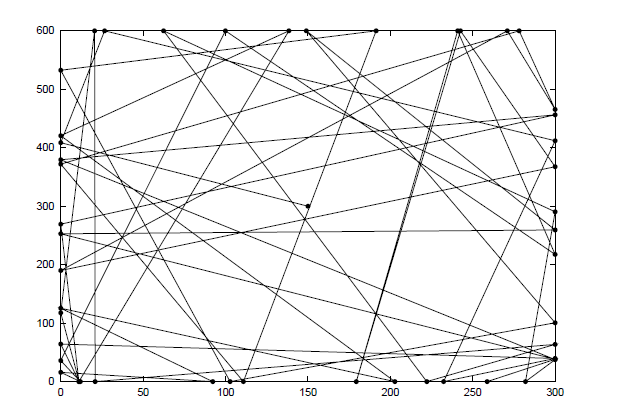
\includegraphics[width=7cm,height=50mm]{../images/randomdirection1.png}
\caption{\label{RandomDirectionFig}Resulting pattern of a MN using the Random Direction Mobility Model}
\end{figure}

\subsubsection{A Boundless Simulation Area}

In this model, there is an important relationship between the old direction and velocity and the current direction and velocity. A velocity vector V = (v,\theta with v a speed and \theta an angular) is used to describe an MN's velocity and a position of an MN is represented as (x,y). The velocity vector and the position are updated in a regular time t. The Boundless Simulation Area Mobility Model is very different that other Mobility Models because here, an MN who reached a border of the simulation area continues his travel and reappears on the opposite side of the simulation area. It results from this that we can consider the simulation area like a torus-shaped, illustrated by the figure \ref{BoundlessFig}. The simulation area is transformed in two step. Firstly, the top border is connected to the bottom border to create a cylinder and then we connected the both open circular ends.

\begin{figure}[h]
\center
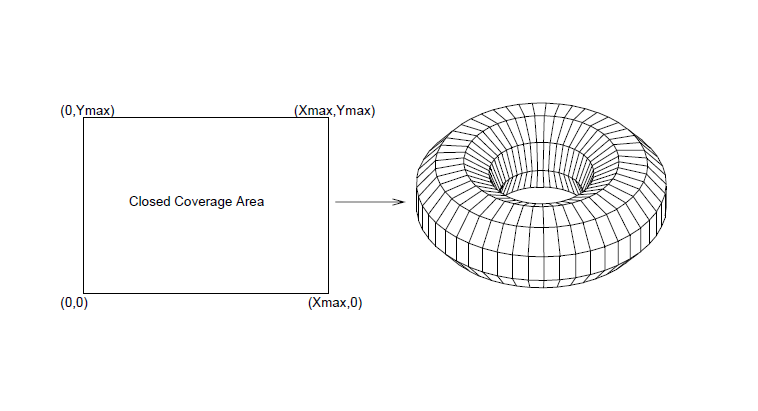
\includegraphics[width=7cm,height=50mm]{../images/boundlessmobilitymodel1.png}
\caption{\label{BoundlessFig}Area mapped to a torus}
\end{figure}


With a speed between 0 and 10 m/s, an angular between 0 and 90 degrees and a time t to 0.1 seconds, the results of the boundless mobility models with this parameters can be seen on the figure \ref{BoundlessFig2}

\begin{figure}[h]
\center
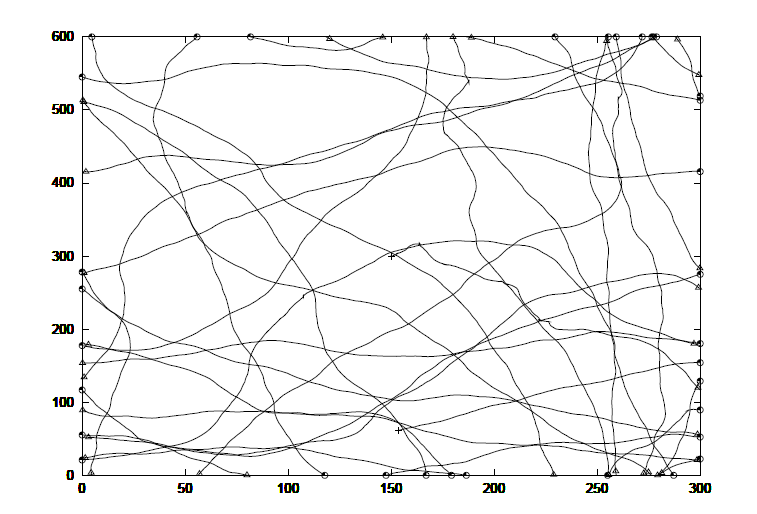
\includegraphics[width=7cm,height=50mm]{../images/boundlessmobilitymodel2.png}
\caption{\label{BoundlessFig2}Resulting pattern of a MN using the Boundless Simulation Area Mobility Model}
\end{figure}

\subsection{Gauss-Markov}

The aim of this model is to be able to adapt with one parameter to different levels of randomness.
Each MN has a current speed and direction. The speed and direction of each MN are updating at a regular time t. At each time t, the next destination and speed are calculated based on the current position of the MN. The MNs are forced away from an edge when the location of a MN is near an border of the simulation area, by modifying the angular direction of the MN like illustrated in the figure \ref{Gauss-MarkovFig1}.

\begin{figure}[h]
\center
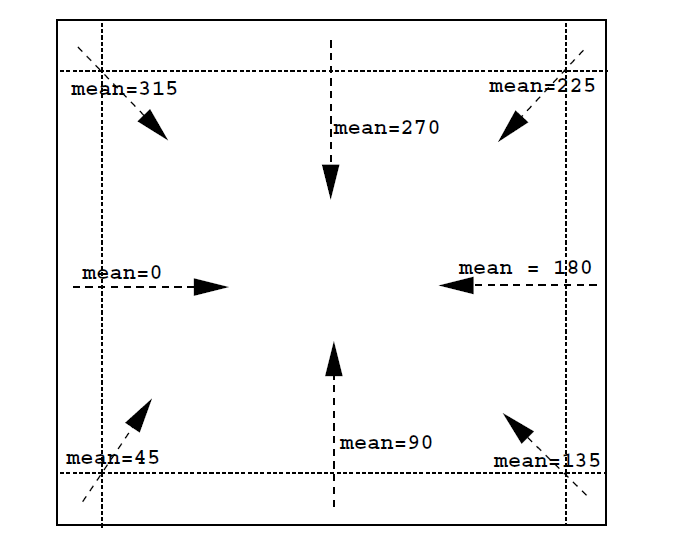
\includegraphics[width=7cm,height=50mm]{../images/gauss-markovmodel1.png}
\caption{\label{Gauss-MarkovFig1}Resulting pattern of a MN using the Boundless Simulation Area Mobility Model}
\end{figure}

In the figure \ref{Gauss-MarkovFig2}, an example of a resulting pattern of a MN using the Gauss-Markov Mobility Model is illustrated. The run takes 1000 seconds and the MN beings at the center of the simulation area. The parameter t is 1 second, the initial angular is 90 degrees and the speed is between 0 and 10 m/s. The Gauss-Markov MM can eliminate the sudden stops and sharp turns encountered in the Random Walk Mobility Model by saved past velocities and directions in order to be able to influence future velocities and directions.

\begin{figure}[h]
\center
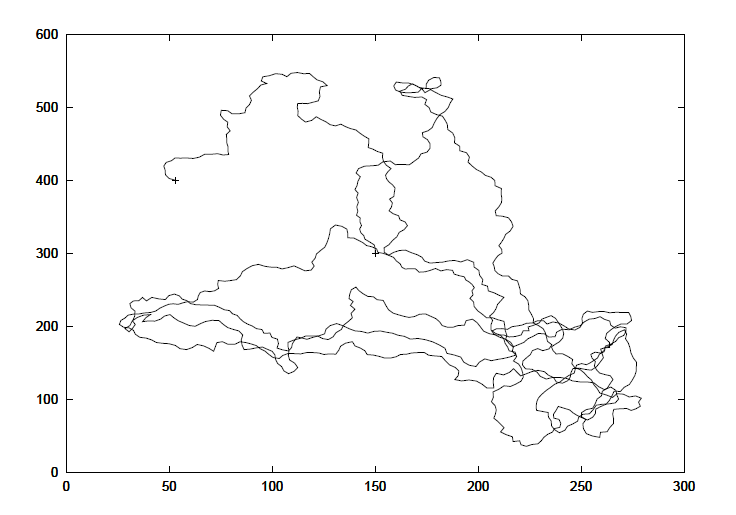
\includegraphics[width=7cm,height=50mm]{../images/gauss-markovmodel2.png}
\caption{\label{Gauss-MarkovFig2}Resulting pattern of a MN using the Boundless Simulation Area Mobility Model}
\end{figure}

\section{Group Mobility Model}

Mobility models that represent mobile nodes whose movements are dependents on each other

\subsection{Reference Point Group Mobility Model}

Group movement are based on the movement of the center of the group. The movement of the group center completely characterizes the motion of the MNs of its group, including their direction and speed. Each MNs randomly and individually move about their own pre-defined reference points, where their movements depend on the group movement. Their position are regularly updated each time t and a new direction is calculated for every MN according to the center of the group.
The figure \ref{RPGMMFig} shows us an illustration of a group of three MNs who move together. The Random Waypoint Mobility Model is used for the random motion of each individual MN in the group and the movement of the center of the group.
In the paper, an application of this model is explained. The RPGMM can be used for example in an avalanche rescue scenario. In a scenario like this, the cooperation between human and canine is essential. We can see the human like the center of the group and the canines are the MNs of the group.


\begin{figure}[h]
\center
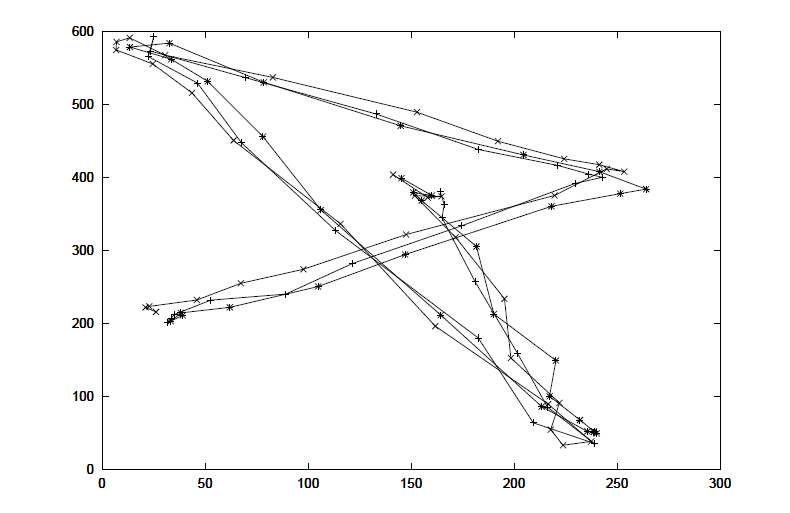
\includegraphics[width=7cm,height=50mm]{../images/rpgmmodel1.png}
\caption{\label{RPGMMFig}Resulting pattern of a MN using the Boundless Simulation Area Mobility Model}
\end{figure}


